\subsection{Land Price Model}
\label{sec:land-price-model} \index{Land Price Model}
\modelsindex
%
The \class{LandPriceModel} predicts prices of land, in particular the
residential and non-residential land value for each member of the given
location set. The prediction is done via a regression procedure and thus,
the model is a child of the \class{RegressionModel} described in
Section~\ref{sec:regression-model}.

\subsubsection{Initialization}
%
The class is initialized by passing the following arguments:
\begin{description}
\item[regression_procedure] - a fully qualified name of the module/class in
  which the regression is implemented (see
  Section~\ref{sec:regression}). Default value is
  ``opus_core.linear_regression''.
\item[filter] - name of a variable/attribute used to filter out elements for
  the regression (applied to both, the \method{run()} and \method{estimate()}
  method). Default value is
  ``urbansim.gridcell.is_in_development_type_group_developable'' which requires an entry 'developable'
  in the table ``develpment_type_groups'' (\ref{sec:development-tables-type-groups}).
\item[submodel_string] - If model contains submodels, this character string
  specifies what attribute of the observation set determines those
  submodels. Default value is ``development_type_id''.
\item[run_config] - A collection of additional arguments that control a
  simulation run. It should be of class \class{Resources}.
\item[estimate_config] - A collection of additional arguments that control an
  estimation run. It should be of class \class{Resources}.
\end{description}
The constructor sets \verb|filter| as a class attribute and calls the parent
constructor (see Initialization in Section~\ref{sec:regression-model}).

\subsubsection{The Run Method}
%
{\it Input}:\\[1mm]
The \method{run()} method takes exactly the same arguments as its parent
class:\\
{\bf specification}, {\bf coefficients}, {\bf dataset}, {\bf index}, {\bf
  chunk_specification}, {\bf data_objects}, and {\bf run_config}.



{\it Algorithm}:\\[1mm]
If \verb|filter| is given in the initialization, \verb|index| is
updated to only those elements for which the value of
attribute/variable \verb|filter| is
larger than zero. It then invokes the \method{run()} method of
\class{RegressionModel} passing all arguments where
\verb|index| is possibly modified. The returned value of this call
is considered to be the prediction of the natural logarithm of total
land value for each element of \verb|dataset| included in
\verb|index|. Each of those values is then exponentiated and split
into residential and non-residential land value, using the attribute
``fraction_residential_land'' (this must be a known
attribute of \verb|dataset|). 
Attributes ``residential_land_value'' and
``nonresidential_land_value'' (which also are expected to be known
attributes of the \verb|dataset|) are modified by
replacing current values with the computed values.

If any of the computed values exceeds the maximal value of float32, a warning
is issued and the value is clipped to the maximal possible value.

{\it Output}:\\[1mm]
The method returns an index of values within \verb|dataset| for which the land
value was modified.

\subsubsection{The Estimate Method}
{\it Input}:\\[1mm]
The \method{estimate()} method takes exactly the same arguments as its parent
class: \\
{\bf specification}, {\bf dataset}, {\bf outcome_attribute}, {\bf index}, {\bf
  procedure}, {\bf data_objects}, and {\bf estimate_config}.

{\it Algorithm}:\\[1mm]
The method applies the \verb|filter| (if given) in the same way as the
\method{run()} method. It then calls the parent method \method{estimate()}
passing all arguments and the possible modified \verb|index|.

{\it Output}:\\[1mm]
The method returns results of \method{estimate()} method of
\class{RegressionModel} (see Section~\ref{sec:regression-model}).

\subsubsection{Model Configuration}
\modelsindex
%
{\em Configuration for Production Run}:\\[1mm]
For a production run of UrbanSim the model is
initialized with default values of the model 
constructor. The \method{run()} method is called by passing the
following arguments:
\begin{description}
\item[specification] - An
\class{EquationSpecification} object created with data from table
``land_price_model_specification''.  
\item[coefficients] - A \class{Coefficients} object created
with data from table ``land_price_model_coefficients''.\modelsindex
\item[dataset] - An instance of class \class{GridcellDataset} created with data
  from table ``gridcells'' (see Section~\ref{sec:gridcell-tables} for the
  table structure).
\item[index] - None. Thus, the model runs on all members of \verb|dataset| which are possibly 
filtered using a filter passed to the constructor (by default ``urbansim.gridcell.is_in_development_type_group_developable'', see
the Initialization paragraph).
\end{description}

\subsubsection{Correct Land Values Model}
\modelsindex
%
\index{Correct Land Values Model}
After the Land Price Model runs at least for 2 years, the production code
invokes every year a model called \class{CorrectLandValue}. This model makes a
correction of the land value to avoid its declination with development type
change.

Its \method{run()} method determines those members of \class{dataset} whose
development type changed and at the same time have lower total land value when
comparing to previous simulated year. Values of the attributes
``residential_land_value'' and ``nonresidential_land_value'' of these members
are replaced by values of the same attributes from previous year. The method
returns an index of the modified \class{dataset} members.

%
\subsection{Development Project Transition Model}
\modelsindex
%
\label{sec:development-project-transition-model}
\index{Development Project Transition Model}
%
The model (implemented in the class \class{DevelopmentProjectTransitionModel}) 
creates development projects in order to match the desired vacancy rates. Each
development project is for a single type of development, e.g.  'industrial' or
'commercial'.  The distribution of project sizes (amount of space, value of
space) is determined by sampling from the projects obtained from the history.

\subsubsection{The Run Method}
%
{\it Input}:
\begin{description}
\item[model_configuration] - a \class{Configuration} object that determines
  project types and settings for each type (see
  Section Model Configuration bellow).
\item[vacancy_table] - a \class{Dataset} object that must have attribute
  ``year'' as the unique identifier and should contain attributes
  ``target_total_residential_vacancy'' and
  ``target_total_non_residential_vacancy''. Those attributes give vacancy
  rates for specific years.
\item[history_table] - a \class{Dataset} object giving historical data of
  development events.
\item[year] - simulated year.
\item[location_set] - a \class{Dataset} object on which vacancies will be
  determined.
\item[resources] - a \class{Resources} object for additional arguments. It can
  contain names of variables that compute the current vacancies per project
  type. Those entry names are composed from the project type and a character
  string `vacant_variable', e.g. for commercial project type the key for this
  argument is ``commercial_vacant_variable''.  Default values for those
  entries are ``urbansim.vacant_'' + project type, e.g.
  ``urbansim.vacant_commercial''.
\end{description}



{\it Algorithm}:~\\[1mm]
The method first determines the target vacancy rates. It distinguishes between
residential and non-residential vacancy rate.  For each project type given in
the \verb|model_configuration|, the method obtains current vacancy in each
location (from \verb|location_set| and the overall vacancy rate). By comparing
the rate with the target vacancy rate, it determines if there is a need for
development and how many units should be developed. If there are units to be
developed, from the historical data it samples sizes of projects so that their
sum gives approximately the desired number of units to be developed. It then
creates an instance of class \class{DevelopmentProjectDataset} for this particular
project type that has unique identifier called ``project_id''. Each project
corresponds to one of the sampled amount of units. This amount is stored in
the new dataset as an attribute given in the entry ``units'' of
\verb|model_configuration| (see below for details). If an attribute called
project type + ``_improvement_value'' is contained in the \verb|location_set|,
an average improvement value is computed over all locations and this project
type and this value is added to each project in the created
\class{DevelopmentProjectDataset}.  Additionally, an attribute of the same name as
the unique identifier of \verb|location_set| is added to the
\class{DevelopmentProjectDataset} and set to 0's (which means that the projects
are unplaced).

{\it Output}:~\\[1mm]
The method returns a dictionary with an entry for each project type containing
the corresponding \class{DevelopmentProjectDataset} object. If no projects were
created for a project type, the corresponding dictionary value is \verb|None|.


\subsubsection{Model Configuration}
\label{sec:DPTM-configuration}
\modelsindex
The \method{run()} method of this class expects a dictionary
\verb|model_configuration| as an argument. This object must contain an entry
``development_project_types'' which is also a dictionary. The name of each
element is a project type and value is again a dictionary. Entries on this
level are ``units'', ``categories'', and ``residential''. Entry ``units''
gives the name of the attribute that determines sizes of projects. An
attribute of the same name must be contained in the \verb|location_set| and in
the dataset with the historical data. Entry ``categories'' determines
categories of a project set. It can be an empty array if categories are not
used. Entry ``residential'' is a boolean value determining if vacancy of this
project type should be compared to the residential vacancy rate or not. In the
latter case, it is compared to the non-residential vacancy rate.

{\em Configuration for Production Run}:\\[1mm]
For a production run of UrbanSim the method \method{run()} is called using the
following arguments:
\begin{description}
\item[model_configuration] - The default configuration for project types in
  \file{general_configuration.py} is \label{page:model-configuration}
\begin{verbatim}
{
    'development_project_types':{
        'residential':{
            'units':'residential_units',
            'categories':array([1,2,3,5,10,20]),
            'residential':True,
            },
        'commercial':{
            'units':'commercial_sqft',
            'categories':1000*array([1, 2, 5, 10]),
            'residential':False,
            },
        'industrial':{
            'units':'industrial_sqft',
            'categories':1000*array([1,2,5,10]),
            'residential':False,
            },
        }
}
\end{verbatim}
\item[vacancy_table] - An object of class \class{TargetVacancyDataset} created
  with data from table ``target_vacancies'' (see
  Section~\ref{sec:table-target-vacancies} for the table structure).
\item[history_table] - An object of class \class{DevelopmentEventDataset} created
  with data from table ``development_event_history'' (see
  Section~\ref{sec:table-development-event-history} for the  table structure).
\item[location_set] - An instance of class \class{GridcellDataset} created with
  data from table ``gridcells'' (see Section~\ref{sec:gridcell-tables} for the
  table structure).
\end{description}



\subsection{Location Choice Model}
\label{sec:location-choice-model}
\index{Location Choice Model}
A location choice model is a choice model where the set of alternatives is a
set of locations.

The class \class{LocationChoiceModel} is a child of \class{ChoiceModel} 
described in Section~\ref{sec:choice-model}. In addition, it allows sampling
of alternatives and filtering alternatives according to a specified filter.

\subsubsection{Initialization}
%
The class is initialized by passing the following arguments:
\begin{description}
\item[location_set] - A dataset of locations to be chosen from.
\item[sampler] - A fully qualified name of the module for sampling
  alternatives. Default value is ``opus_core.samplers.weighted_sampler''. If
  this argument is set to None, no sampling is performed.
\item[utilities] - A fully qualified name of the module for computing utilities
  (see Section~\ref{sec:utilities}). Default value is
  ``opus_core.linear_utilities''.
\item[probabilities] - A fully qualified name of the module for computing
  probabilities (see Section~\ref{sec:probabilities}). Default value is
  ``opus_core.mnl_probabilities''.
\item[choices] - A fully qualified name of the module for determining
  final choices (see Section~\ref{sec:choices}). Default value is
  ``opus_core.random_choices''.
\item[interaction_pkg] - This argument is only relevant if there is an
  explicit implementation of an interaction dataset that corresponds to
  interaction between agents and choices (such as those from
  Table~\ref{tab:urbansim-interaction-datasets}). It then determines the
  package in which the module lives. Default value is
  ``urbansim.datasets''. 
\item[filter] - It is either a string specifying an attribute name of the
  filter, or a 1D/2D array giving the filter directly, or a dictionary
  specifying filter for each submodel. If it is None (default), no filter is
  applied.
\item[submodel_string] - If model contains submodels, this character string
  specifies what agent's attribute determines those submodels. If it is None
  (default), no division into submodels is applied.
\item[run_config] - A collection of additional arguments that control a
  simulation run. It should be of class \class{Resources}.
\item[estimate_config] - A collection of additional arguments that control an
  estimation run. It should be of class \class{Resources}.
\end{description}
The method calls the constructor of its parent class. Then, it creates a
\class{Sampler} object from the argument \verb|sampler| using
\class{SamplerFactory}. It sets value of the argument \verb|filter| as a class
property \verb|filter|

%
\subsubsection{The Run Method}
%
The \method{run()} method runs the simulation of location choice model on basis
of a given specification and coefficients.

{\it Input}:\\[1mm]
It takes the same arguments as the \method{run()} method of its parent (see
Section~\ref{sec:choice-model} for more details): \\
{\bf specification}, {\bf coefficients}, {\bf agent_set}, {\bf agents_index},
{\bf chunk_specification}, {\bf data_objects}, and {\bf run_config}.

{\it Algorithm}:\\[1mm]
The model is processed in chunks. The \method{run_chunk()} method moves
the agents out of their locations, i.e. the values of an
\verb|agent_set| attribute of the same name as the unique identifier of
\verb|location_set| is set to $-1$ for each agents of the currently processed
chunk. If \verb|agent_set| does not have this attribute, it is appended to it.

If an entry ``compute_capacity_flag'' is given in \verb|run_config| and its
value is True, an entry ``capacity_string'' is expected in \verb|run_config|
which gives the name of attribute/variable of \verb|location_set| that
determines capacity for each location. In such a case, after removing agents
from their locations, the capacity is computed using method
\method{determine_units_capacity()}. Note that by removing agents of only the
current chunk from their locations, the capacity is influenced by only those
agents. Each chunk then see the state of the world updated by all previously
running chunks.

The capacity values are used as weights of locations in the case of sampling.
They are multiplied by the filter given in the initialization.  The
model then invokes sampling of alternatives by calling the
\method{run()} method of the sampler class, passing the possibly filtered
weights. The parent class then takes care of creating the interaction set, for
agents of the corresponding chunk and possibly sampled alternatives and of
running the \verb|upc_sequence|. If \verb|run_config| includes an entry
``correct_sampling_bias'' that is set to True, the method performs a bias
correction for non-uniform sampling in the multinomial logit computation.

The location IDs that agents chose in the choice process are stored
in the \verb|agent_set| attribute specifying the location.

{\it Output}:\\[1mm]
The method returns an array of size \verb|agents_index|,
representing the location IDs that agents (elements of
\verb|agent_set| determined by \verb|agents_index|) made. Agents
whose choice is less equal zero were not included in the choice
process, for example because they do not belong to any submodels
given in the specification.


\subsubsection{The Estimate Method}
%
{\it Input}:~\\[1mm]
The \method{estimate()} method takes the same arguments as its parent class:\\
{\bf specification}, {\bf agent_set}, {\bf agents_index}, {\bf procedure},
{\bf data_objects}, and {\bf estimate_config}.

{\it Algorithm}:\\[1mm]
As in the \method{run()} method, if ``compute_capacity_flag'' is given in
\verb|estimate_config| and its value is True, an entry ``capacity_string'' is
expected in \verb|estimate_config| which gives the name of attribute/variable
of \verb|location_set| that determines capacity for each location. In such a
case, the capacity is computed using method
\method{determine_units_capacity_for_estimation()}.

The weights for sampling alternatives are determined by an optional entry
``weights_for_estimation_string'' in \verb|estimate_config| which should be an
attribute/variable name of \verb|location_set|. They are multiplied by the
given \verb|filter| (if any) and as in the case of the \method{run()} method,
sampling is performed using those weights. The parent class performs then the
estimation. If \verb|estimate_config| includes an entry
``correct_sampling_bias'' that is set to True, the method performs a bias
correction for non-uniform sampling by adding an appropriate column to the
data that enter the estimation.

{\it Output}:\\[1mm]
The method passes the return values of its parent method \method{estimate()},
i.e. a tuple of the created \class{Coefficient} object and a
dictionary with entries for each submodel equals a dictionary returned by the
\verb|run()| method of \verb|procedure| for that submodel.

%
\subsubsection{Model Configuration}
\modelsindex
%
The arguments \verb|run_config| and \verb|estimate_config| are collections of
parameters that control the \method{run()} and \method{estimate()} method,
respectively. In addition to the mentioned entries ``compute_capacity_flag'',
``capacity_string'' and ``correct_sampling_bias'', they can contain entries
``sample_proportion_locations'' and ``sample_size_locations''. Both entries
control the size of sampled alternatives, the first one as a relative number,
the latter one as an absolute number. The latter one has a priority over the
first one.

As mentioned above, \verb|estimate_config| can also contain an entry ``weights_for_estimation_string''.


\subsection{Development Project Location Choice Model}
\label{sec:development-project-lcm}
\index{Development Project Location Choice Model}
%
The Development project location choice model simulates a process where
development projects of a specific type choose locations to be placed into.
The class \class{DevelopmentProjectLocationChoiceModel} is a child of
\class{LocationChoiceModel} described in
Section~\ref{sec:location-choice-model}.

\subsubsection{Initialization}
%
The class is initialized by passing the following arguments:
\begin{description}
\item[location_set] - A dataset of locations to be chosen from.
\item[project_type] - A character string determining the type of the projects
  for this model. 
\item[units] - A character string giving the name of the attribute that
  determines sizes of projects.
\item[developable_maximum_unit_variable_full_name] -  A character string determining
  which Opus variable to use for the maximum developable units.
\item[developable_minimum_unit_variable_full_name] -  A character string determining
  which Opus variable to use for the minimum developable units.
\item[model_name] - An optional argument giving the model name.
\item[+] all remaining arguments from the constructor of
  \class{LocationChoiceModel}. 
\end{description}
The \verb|location_set| is expected to have a variable
``developable_minimum_''+\verb|units| and ``developable_maximum_''+\verb|units|
implemented in the given \verb|opus_package|.


\subsubsection{The Run Method}
%
{\it Input}:\\[1mm]
It takes the same arguments as the \method{run()} of its parent: \\
{\bf specification}, {\bf coefficients}, {\bf agent_set}, {\bf agents_index},
{\bf chunk_specification}, {\bf data_objects}, and {\bf run_config}.

The \verb|agent_set| is expected to be an instance of
\class{DevelopmentProjectDataset}. It is assumed that initially all projects are
unplaced.

{\it Algorithm}:\\[1mm]
The model must be set to use capacity (via entries ``compute_capacity_flag''
and ``capacity_string'' in \verb|run_config|).  The capacity attribute is
considered as a variable that is 1 for locations that are developable for this
particular project type, otherwise 0. This means that no more than one project
of the same type can occupy one location. The method
\method{determine_units_capacity()} assures that locations taken in previous
chunks are marked as taken.

The weight array for sampling is constructed in each chunk by combining
information about project sizes and minimum and maximum developable units in
each location.  Thus, the weight array is a 2-d array which implies that
different projects have different weights for the same locations, depending on
their size. The dimension of the location axis of this array is for memory
reasons reduced to only locations that are developable. No additional
filtering is done (the model sets the class property \verb|filter| to
\verb|None|).

The class overwrites the method \verb|get_agents_order()| in a way that it
sorts the agents according to their sizes in descending order. This means that
larger projects enter the choice process first.

The \method{run()} method proceeds otherwise as defined in the parent class.

{\it Output}:~\\[1mm]
It returns results of its parent class.

\subsubsection{The Estimate Method}
%
The \method{estimate()} method is identical to its parent method
\method{estimate()}.


\subsubsection{Creators}
%
The model can be created using pre-defined creators in \package{urbansim}.
The class\\
\class{DevelopmentProjectLocationChoiceModelCreator} sets useful default
values for arguments of the constructor, \verb|run_config| and
\verb|estimate_config|. The model is by default initialized with:
\begin{description}
\item[sampler] - ``opus_core.samplers.weighted_sampler''
\item[utilities] - ``opus_core.linear_utilities''
\item[probabilities] - ``opus_core.mnl_probabilities''
\item[choices] - ``urbansim.first_agent_first_choices'' (see
  Section~\ref{sec:urbansim-choices})
\item[submodel_string] - ``size_capacity''
\end{description}
Entries of \verb|run_config| are set as to:
\begin{verbatim}
{   "compute_capacity_flag": True,
    "sample_size_locations": 10,
    "correct_sampling_bias": False,
    "capacity_string": "urbansim.gridcell.is_developable_for_%s" % units }
\end{verbatim}
The variable \verb|units| in the last line is taken from a model configuration
that is passed to the creator in an entry ``units'' of the corresponding
project type (see model configuration on
page~\pageref{page:model-configuration}).

Entries of \verb|estimate_config| are set as to:
\begin{verbatim}
{   "estimation": "opus_core.bhhh_mnl_estimation",
    "sample_size_locations": 10,
    "estimation_size_agents": 1.0,
    "correct_sampling_bias": False  }
\end{verbatim}


\class{DevelopmentProjectLocationChoiceModelCreator} is used by
\begin{itemize}
\item \class{DevelopmentProjectCommercialLocationChoiceModelCreator} 
\item \class{DevelopmentProjectIndustrialLocationChoiceModelCreator} 
\item \class{DevelopmentProjectResidentialLocationChoiceModelCreator} 
\end{itemize}
which set in addition the appropriate type of projects for which the model 
should run.

\subsubsection{Model Configuration}
\modelsindex
%
{\em Configuration for Production Run}:\\[1mm]
The production run of UrbanSim is configured with three development project
types: ``residential'', ``commercial'', and ``industrial''. Thus, there are
three instances of the model, each initialized with the particular project
type and a \class{GridcellDataset} as \verb|location_set|.  Each of the models 
runs only if the Development Project Transition Model returns some projects
for the project type, i.e. the output value for this particular project type
is not None.  The \method{run()} method of each of the model is called by
passing the following arguments:
\begin{description}
\item[specification] - An
\class{EquationSpecification} object created with data from table
``\%s_development_location_choice_model_specification''.  
\item[coefficients] - A \class{Coefficients} object created
with data from table ``\%s_development_location_choice_model_coefficients''.\modelsindex
\item[agent_set] - A \class{DevelopmentProjectDataset} returned by the Development
  Project Transition Model in its entry for this particular project type.
\end{description}
The ``\%s'' in the above character strings are replaced by project type.

%
\subsection{Development Event Transition Model}
\modelsindex
%
\label{sec:development-event-transition-model}
\index{Development Event Transition Model}
%
The model creates for each location a development event, which is a collection
of development projects of different type (e.g. commercial, residential,
industrial) for this location. This model is not estimated and contains only a
method \method{run()}.

%
\subsubsection{The Run Method}
%
{\it Input}:
\begin{description}
\item[projects] - a dictionary where key is the type of development
  project and value is an instance of \class{DevelopmentProjectDataset} for that
  particular project type.
\item[types] - a list of project types which the resulting event should
  consist of.
\item[units] - a list of attribute names (defined as dataset qualified names)
  that determine the units for each project type (e.g. ``commercial_sqft'' for
  copmmercial type or ``residential_units'' for residential type). The
  ordering in the list must correspond to the ordering in \verb|types|.
\item[year] - an integer indicating for which year this events are
  created. Default value is 0.
\item[location_id_name] - name of the attribute that determines
  locations. Default value is ``grid_id''.
\end{description}

{\it Algorithm}:\\[1mm]
It generates a distinct set of all locations in which at least one project is
located. It creates a \class{DevelopmentEventDataset} of size of number of those
locations. It has an attribute given in \verb|location_id_name| with id values
of the locations. Furthermore, it has all attributes given in the argument
\verb|units|. Values for each these attributes are the sums of values of the
attribute of the same name in the corresponding project dataset over the
corresponding locations. It also has an attribute ``scheduled_year'' with the
same value for each location, namely the one given in the argument
\verb|year|. Additional attributes \verb|type| + ``_improvement_value''
contain the sum of the project set attribute ``improvement_value'' over the
corresponding locations.

{\it Output}:~\\[1mm]
The model returns an instance of \class{DevelopmentEventDataset}.

\subsubsection{Model Configuration}
\modelsindex
%
{\em Configuration for Production Run}:\\[1mm]
In a production run of UrbanSim, the \method{run()} method is called by
passing the following arguments:
\begin{description}
\item[projects] - A dictionary that results from a run of the Development
  Project Transition Model, and is (possibly) modified by runs of all three
  Development Project Location Choice Models. 
\item[types] - A list of project types for which the Development Project
  Location Choice Model has run, i.e. for which there are projects to be
  developed.
\item[units] - A list of ``units'' entries from model configuration in
  \file{general_configuration.py} (see page~\pageref{page:model-configuration}) for which the
  Development Project Location Choice Model has run, i.e. that correspond to
  \verb|types|.
\item[year] - The simulated year.
\end{description}


%
\subsection{Events Coordinator}
\label{sec:events-coordinator}
\index{Events Coordinator}
%
The class \class{EventsCoordinator} updates a location set to reflect changes
that are contained in the output of the Development Event Transition Model. 
There is no \method{estimate()} method for this model. 
%
\subsubsection{The Run Method}
%
{\it Input}:
\begin{description}
\item[model_configuration] - a \class{Configuration} object that determines
  project types and settings for each type (see Model Configuration of
  Section~\ref{sec:development-project-transition-model}).
\item[location_set] - a \class{Dataset} object to be updated.
\item[development_event_set] - a \class{DevelopmentEventDataset} with development
  events to be used to update the locations.
\item[development_type_set] - an object of class \class{DevelopmentTypeDataset}.
\item[current_year] - an integer value determining the year of events by
  which the locations are updated.
\end{description}

{\it Algorithm}:\\[1mm]


{\it Output}:~\\[1mm]
Returns a tuple of indices of locations that were modified, and indices of
development events that were processed.

\subsubsection{Model Configuration}
\modelsindex
%
{\em Configuration for Production Run}:\\[1mm]
For a production run of UrbanSim the method \method{run()} is called using the
following arguments:
\begin{description}
\item[model_configuration] - The model configuration for project types from
  \file{general_configuration.py} as shown on page~\pageref{page:model-configuration}.
\item[location_set] - An instance of class \class{GridcellDataset} created with
  data from table ``gridcells'' (see Section~\ref{sec:gridcell-tables} for the
  table structure) and (possibly) modified by previous models. 
\item[development_event_set] - Result of a Development Event Transition Model 
  run.
\item[development_type_set] - An object of class \class{DevelopmentTypeDataset}
  created with data from table ``development_types'' and
  ``development_type_group_definitions'' (see
  Section~\ref{sec:development-tables} for the tables structure).
\item[current_year] - The current year of the simulation.
\end{description}

%
\subsection{Residential Land Share Model}
\modelsindex
%
\label{sec:residential-land-share-model}
\index{Residential Land Share Model}

Residential land share model (implemented in class
\class{ResidentialLandShareModel}) predicts what fraction of each location is
residential land. It is a \class{RegressionModel} 
(Section~\ref{sec:regression-model}) with an only method overwritten, the
\method{run()} method.

\subsubsection{The Run Method}
%
{\it Input}:\\[1mm]
It takes the same arguments as the \method{run()} of its parent: \\
{\bf specification}, {\bf coefficients}, {\bf dataset}, {\bf index}, {\bf
  chunk_specification}, {\bf data_objects}, and {\bf run_config}.

{\it Algorithm}:\\[1mm]
The \method{run()} method of \class{RegressionModel} is invoked in order to
obtain a regression outcome $y$. If the run
was successful, the resulting quantity $y'$ is computed as
\[
y' = \frac{e^y}{1+e^y}
\]
$y'$ is an array of values for each member of \verb|dataset| given by
\verb|index|. Those values are stored in the attribute given by the class
property \verb|attribute_to_modify|. This is by default
``fraction_residential_land''. If such attribute does not exists in the
\verb|dataset|, it is created.

{\it Output}:\\[1mm]
The method returns $y'$.

\subsubsection{Model Configuration}
\modelsindex
%
{\em Configuration for Production Run}:\\[1mm]
For a production run of UrbanSim the method \method{run()} is called only if
the Events Coordinator actually changed any locations.  The following
arguments are passed to the run:
\begin{description}
\item[specification] -  An
\class{EquationSpecification} object created with data from table
``residential_land_share_model_specification''. 
\item[coefficients] - A \class{Coefficients} object created
with data from table ``residential_land_share_model_coefficients''.\modelsindex
\item[dataset] - An instance of class \class{GridcellDataset} that was passed to
  the Events Coordinator.
\item[index] - Indices of the gridcells that were changed by the Events
  Coordinator, i.e. the first element of its output tuple.
\end{description}

%
\subsection{Household Transition Model}
\modelsindex
%
\label{sec:household-transition-model}
\index{Household Transition Model} The class \class{HouseholdTransitionModel} 
creates and removes households to and from given household set according to
the joint distribution of their characteristics. The total number of
households is controlled by given annual control totals.

\subsubsection{The Run Method}
%
{\it Input}:
\begin{description}
\item[year] - an integer indicating the simulated year.
\item[household_set] - an instance of \class{Dataset} that contains some
  specific attributes (see description of the algorithm bellow).
\item[control_totals] - an instance of \class{ControlTotalDataset} initiated for
  the dataset ``household''. It must have at least attributes
  ``total_number_of_households'' and ``year'' which give the control totals
  for specific years. Optionally, it can contain other attributes whose
  combinations determine groups for the control totals.  These are e.g.
  ``age_of_head'', ``income'', ``persons'', ``cars'', ``children'',
  ``race_id'', ``workers''. Each value of such attribute is the corresponding
  group index (starting from zero) for this characteristics from the argument
  \verb|characteristics| (see below). The unique identifier of this dataset 
  should consist of all attributes but the ``total_number_of_households'' (for
  details see Section ``annual_household_control_totals''
  in~\ref{sec:household-tables-ahct}).
\item[characteristics] - an instance of class
  \class{HouseholdCharacteristicDataset} that specifies grouping of
  characteristics.  It must have three attributes: ``characteristic'', ``min''
  and ``max''.  Values of the ``characteristic'' attribute should match the
  names of the existing optional attributes of \verb|control_totals|, but they
  can be also other names. ``min'' and ``max'' determine group boundaries for
  each characteristics (for details see Section
  ``household_characteristics_for_ht'' in~\ref{sec:household-tables-char-for-ht}). If
  there is a characteristics missing that is contained in
  \verb|control_totals|, the grouping is assumed to be $[0,1), [1,2), [2,3)$,
  etc.
\item[resources] - additional \class{Resources} for controlling the
  simulation run. The argument is not used in this version of the model. 
\end{description}

{\it Algorithm}:~\\[1mm]
The optional attributes in \verb|control_totals| are called 'marginal'
characteristics, the remaining characteristics from the dataset 
\verb|characteristics| are called 'scaled' characteristics. The given
\verb|household_set| must contain the union of the marginal and scaled
characteristics as its primary attributes. \primaryattributesindex

The combination of all marginal characteristics and the grouping within each
of them determines distinct marginal bins.  The method iterates over those
bins. In each iteration the number of households is determined whose
properties match the characteristics of the bin. This number is compared to
the control total for this bin. If the difference $d$ is positive, new
households are created, if it is negative, households are removed, if it is
zero, nothing is done.

When creating households, the method samples $d$ bins from the scaled
characteristics bins that this marginal bin applies to. These represent
categories to which the $d$ new households belong to. For each new household
the value of each characteristics is randomly sampled between the category
minimum and maximum (as an integer value). There are two exceptions:
characteristics ``age_of_head'' is never smaller than 15. Sampled values of
the characteristics ``income'' are rounded to the nearest 10.

To remove households, first unplaced households from the bin are removed. If
the number $n_u$ of those unplaced households is larger than $d$, only $d$
households are randomly sampled for deletion. If $n_u$ is smaller than $d$,
then $d-n_u$ households from the set of placed households of that bin are
randomly sampled and deleted. Households are considered as unplaced if their
attribute given by the class property \verb|location_id_name| (which is by
default ``grid_id'') is smaller equal zero.

{\it Output}:~\\[1mm]
The method returns the total difference between the sizes of the household
dataset after and before the model run. Thus, a positive value means that in
total there were more households added than removed, a negative value means
the opposite.

%
\subsubsection{Example}
%
Consider the following example. We have two marginal characteristics defined
in the control totals - persons and income. The dataset \verb|characteristics|
defines three categories - persons (3 groups), income (2 groups) and age of
head (3 groups). A combination of those groups divides the space of households
characteristics into 18 groups in total, as shown in
Figure~\ref{fig:htm-example}.

\begin{figure}
\begin{center}
%begin{latexonly}
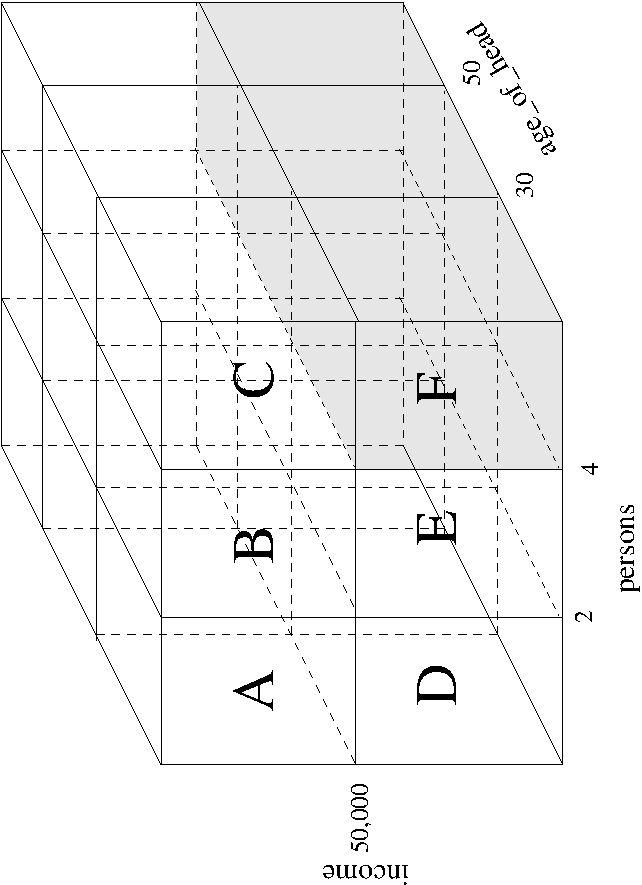
\includegraphics[scale=0.5, angle=-90]{images/htmexample.pdf}
%end{latexonly}
\caption{\label{fig:htm-example}\small Example of dividing household
  characteristics into bins.}
\htmlonly{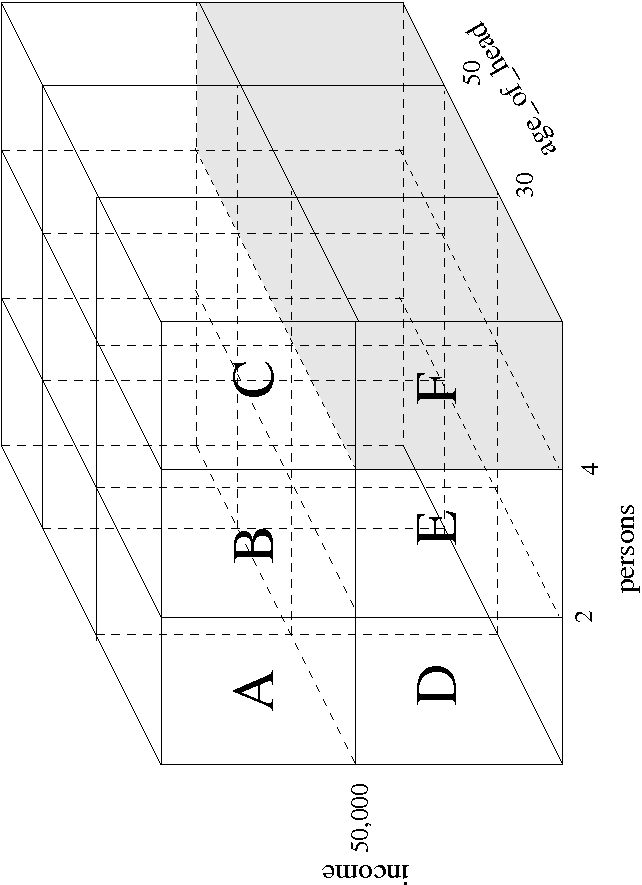
\includegraphics[scale=0.5, angle=-90]{images/htmexample.jpg}}
\end{center}
\end{figure}

The table for the control totals dataset can be
defined as follows:
\begin{verbatim}
year       persons      income     total_number_of_households
2006         0             0                100100
2006         1             0                230000
2006         2             0                 10000
2006         0             1                150000
2006         1             1                250000
2006         3             1                  5000
2007         0             0                110000
  .
  .
  .
\end{verbatim}
The characteristics table defines the groups of each characteristics:
\begin{verbatim}
characteristic      min        max
persons               0          2
persons               2          4
persons               4         -1
income                0      49999
income            50000         -1
age_of_head           0         29
age_of_head          30         49
age_of_head          50         -1
\end{verbatim}
Note that $-1$ stands for $\infty$. The values in the control totals table
denotes the index (starting from 0) of the particular group within the
characteristics table. E.g. the first line in the control totals table refers
to the persons group $[0,2]$ and income group $[0,49999]$.

The model iterates over bins defined by the marginal characteristics. In this
case, it would iterate over the 6 groups marked by A,B,C,D,E,F in
Figure~\ref{fig:htm-example}, it would then determine the number of households
that belong to each group in terms of their characteristics and compare it
with the control total for that group. If for example in bin F (shaded area in
the figure) there are 10 households to be created, the model would randomly
sample (with replacement) 10 bins from the 3 bins within F (formed by groups
on the axis ``age_of_head''), weighted by the number of existing households in
those bins.  These are categories of the 10 new households. Then for each of
the 10 households it would randomly sample the actual value of each
characteristics.  For example, for the very front cube of F, it would sample
income between 0 and $49,999$ (rounded to the nearest 10), number of persons
between 4 and 8\footnote{When a maximum is set to $\infty$, we replace it by a
  reasonable maximum for sampling, which is two times the category range.}
and age of head between 15 and 29.  If the difference between control total
and the number of households in F would call for removing households, the
model would randomly sample households belonging to F regardless to which bin
within F they belong.

\subsubsection{Model Configuration}
\modelsindex
%
{\em Configuration for Production Run}:\\[1mm]
In a production run of UrbanSim, the model runs with the following arguments:
\begin{description}
\item[year] - The current year of the simulation.
\item[household_set] - A \class{HouseholdDataset} object created with data from
  table ``households'' (see Section~\ref{sec:household-tables}
  for the table structure).
\item[control_totals] - A \class{ControlTotalDataset} object inititated with the
  argument \verb|what=|``household'' that reads data from table
  ``annual_household_control_totals'' (see Section~\ref{sec:household-tables}
  for the table structure).
\item[characteristics] - A \class{HouseholdCharacteristicDataset} object created
  with data from table ``household_characteristics_for_ht'' (see
  Section~\ref{sec:household-tables} for the table structure).
\end{description}


%
\subsection{Employment Transition Model}
\modelsindex
%
\label{sec:employment-transition-model}
\index{Employment Transition Model}

The class \class{EmploymentTransitionModel} creates and removes jobs to and
from given job set according to a job distribution over employment sectors.
The total number of jobs is controlled by given annual control totals. It
distinguishes between home based and non-home based jobs.

The algorithm is a simplification of the Household Transition Model. There are
no scaled characteristics and the only marginal characteristics are sector
identifiers.

\subsubsection{The Run Method}
%
{\it Input}:
\begin{description}
\item[year] - an integer indicating the simulated year.
\item[job_set] - an instance of \class{Dataset} that contains some
  specific attributes (see description of the algorithm bellow).
\item[control_totals] - an instance of \class{ControlTotalDataset} initiated for
  the dataset ``employment''. It must have at least attributes ``sector_id'',
  ``total_home_based_employment'', ``total_non_home_based_employment'' and
  ``year'' which specify the annual control totals per sector and employment
  type.  The unique identifier of this dataset should be ``year'' and
  ``sector_id'' (for details see Section ``annual_employment_control_totals''
  in~\ref{sec:employment-tables}).
\item[job_building_types] - an instance of class \class{Dataset} that contains unique 
building types of jobs. It must contain an attribute 'home_based' determining which 
of the building types are home based (see ``job_building_types'' in~\ref{sec:employment-tables}).
 \item[data_objects] - a dictionary containing other datasets and arguments
  needed for computing variables.
\item[resources] - additional \class{Resources} for controlling the
  simulation run. The argument is not used in this version of the model. 
\end{description}


{\it Algorithm}:~\\[1mm]
The \verb|job_set| is required to have a primary attribute \primaryattributesindex
``building_type'' with values that correspond to values of the unique identifier of \verb|job_building_types|.
The algorithm invokes a computation of variables
``is_in_employment_sector_$n$_home_based'' and
``is_in_employment_sector_$n$_non_home_based'' implemented in the package
given by the class property \verb|variable_package| (by default
``urbansim''). $n$ in the variable names is the sector id. If you use
the default \package{urbansim} implementation of those variables, they require
a primary attributes \primaryattributesindex ``home_based'' of the dataset \verb|job_building_types|
and a primary attribute ``sector_id'' of \verb|job_set|. Each job is set to be home based if its building 
type is home based, otherwise the job is non-home based.  

The method iterates over sectors given in \verb|control_totals|. For each
sector it determines the number of jobs of that sector that are home based
(non-home based) using the above variables. It then compares those numbers to
the control totals.  If the difference $d_h$ ($d_{nh}$) is positive, new home
based (non-home based) jobs are created, if it is negative, home based
(non-home based) jobs are removed, if it is zero, nothing is done.

Jobs that are created get the corresponding values for the attribute
``sector_id''. For each combination of (sector id, home based) and (sector id, non-home based) 
it is determined, if there are any jobs of this group
previously available. In such a case, the distribution of ``building_type'' among those jobs is
determined and the values for ``building_type'' of the new jobs are sampled
from this distribution. If there are no existing jobs in this group, it is
sampled from the ``building_type'' distribution obtained over all home based
(non-home based) jobs, regardless of the sector id.

To remove home based (non-home based) jobs from a sector, first unplaced home
based (non-home based) jobs of this sector are removed. If the number $n_{h_u}$
($n_{nh_u}$) of those unplaced jobs is larger than $d_h$ ($d_{nh}$), only
$d_h$ ($d_{nh}$) jobs are randomly sampled for deletion. If $n_{h_u}$
($n_{nh_u}$) is smaller than $d_h$ ($d_{nh}$), then $d_h-n_{h_u}$
($d_{nh}-n_{nh_u}$) jobs from the set of placed jobs of that sector are
randomly sampled and deleted. Jobs are considered as unplaced if their
attribute given by the class property \verb|location_id_name| (which is by
default ``grid_id'') is smaller equal zero.

{\it Output}:~\\[1mm]
The method returns the total difference between the sizes of the job
dataset after and before the model run. Thus, a positive value means that in
total there were more jobs added than removed, a negative value means
the opposite.

\subsubsection{Model Configuration}
\modelsindex
%
{\em Configuration for Production Run}:\\[1mm]
In a production run of UrbanSim, the model runs with the following arguments:
\begin{description}
\item[year] - The current year of the simulation.
\item[job_set] - A \class{JobDataset} object created with data from
  table ``jobs'' (see Section~\ref{sec:employment-tables}
  for the table structure).
\item[control_totals] - A \class{ControlTotalDataset} object initiated with the
  argument \verb|what=|``employment'' that reads data from table
  ``annual_employment_control_totals'' (see
  Section~\ref{sec:employment-tables} for the table structure).
\item[job_building_types] - A \class{JobBuildingTypeDataset} created with data from table 
``job_building_types'' (see Section~\ref{sec:employment-tables}
  for the table structure).
\end{description}



%
\subsection{Agent Relocation Model}
\modelsindex
%
\label{sec:agent-relocation-model}
\index{Agent Relocation model}

The class \class{AgentRelocationModel} determines which members of the given
set of agents should be relocated. This is done on basis of given
probabilities. Additionally, the way how to choose the agents can be given by
passing a \class{Choices} object.

%
\subsubsection{Initialization}
%
The class is initialized by passing the following arguments:
\begin{description}
\item[probabilities] - A fully qualified name of the module that implements
  computing relocation probabilities. The module should be a child of the
  \package{opus_core} class \class{Probabilities}.
\item[choices] - A fully qualified name of the module that implements choosing
  agents for relocation according to given probabilities. The module should be
  a child of the \package{opus_core} class \class{Choices}.  Default value is
  ``opus_core.random_choices'' (see Section~\ref{sec:choices}).
\item[location_id_name] - Name of the attribute that specifies locations. It
  must be a primary attribute \primaryattributesindex of the agent set. Default value is
  ``grid_id''.
\item[model_name] - Name of the model. Default value is ``Agent Relocation
  Model''. 
\end{description}
The initialization method creates a class attribute \verb|upc_sequence|, using
the passed arguments \verb|probabilities| and \verb|choices|. It is an object
of class \class{upc_sequence} where the utilities component is set to None
(see Section~\ref{sec:upc-sequence}).

%
\subsubsection{The Run Method}
%
{\it Input}:
\begin{description}
\item[agent_set] - A \class{Dataset} object containing agents to be relocated.
\item[resources] - An instance of class \class{Resources} which is a
  collection of additional arguments and objects that will be passed to the
  \verb|upc_sequence| run.
\end{description}

{\it Algorithm}:~\\[1mm]
The method appends \verb|agent_set| into \verb|resources| and invokes the
\method{run()} method of \verb|upc_sequence|, passing \verb|resources| as
argument. The \verb|upc_sequence| runs the probabilities component and the
choices component and it is expected to return an array of zeros for agents
not to be relocated, and ones for agent to be relocated. The distinct values
of indices of the ``to be relocated'' agents joined with indices of all
unplaced agents is the resulting array of agents to be relocated. As unplaced
agents are considered agents that have value smaller equal 0 for the attribute
given in \verb|location_id_name| passed to the constructor.

{\it Output}:~\\[1mm]
The method returns the resulting array of indices of all agents to be
relocated.

%
\subsubsection{Creators}
%
There are two pre-defined creators in \package{urbansim}. Their method
\method{get_model()} returns an instance of
\class{AgentRelocationModel} with the following default settings:
\begin{itemize}
\item \class{HouseholdRelocationModelCreator} - sets the argument
  \verb|probabilities| to ``urbansim.household_relocation_probabilities''
  (see Section~\ref{sec:urbansim-probabilities}) and \verb|model_name| to
  ``Household Relocation Model''. 
\item \class{EmploymentRelocationModelCreator} - sets the argument
  \verb|probabilities| to
  ``urbansim.employment_relocation_probabilities'' (see
  Section~\ref{sec:urbansim-probabilities}) and \verb|model_name| to
  ``Employment Relocation Model''.  
\end{itemize}

%
\subsubsection{Model Configuration}
\modelsindex
%
{\em Configuration for Production Run}:
\begin{itemize}
\item To run a {\bf Household Relocation Model} in a production run, the
  \class{HouseholdRelocationModelCreator} is used to create an instance of the
  \class{AgentRelocationModel}. Additionally, it creates an instance of
  \class{RateDataset} initialized with the argument \verb|what=|''households''
  which reads data from table ``annual_relocation_rates_for_households'' (see
  Section~\ref{sec:household-tables} for the table structure). This object is
  put into {\bf resources} which is passed to the \method{run()} method of
  the model. As {\bf agent_set} the production code passes a
  \class{HouseholdDataset} object that was (possibly) used and modified by the
  Household Transition Model. 
\item To run a {\bf Employment Relocation Model}, the
  \class{EmploymentRelocationModelCreator} is used to create an instance of the
  \class{AgentRelocationModel}. Additionally, it creates an instance of
  \class{RateDataset} initialized with the argument \verb|what=|''jobs''
  which reads data from table ``annual_relocation_rates_for_jobs'' (see
  Section~\ref{sec:employment-tables} for the table structure). This object is
  put into {\bf resources} which is passed to the \method{run()} method of
  the model. As {\bf agent_set} the production code passes a
  \class{JobDataset} object that was (possibly) used and modified by the
  Employment Transition Model. 
\end{itemize}

%
\subsection{Agent Location Choice Model}
\modelsindex
%
\label{sec:agent-lcm}
\index{Agent Location Choice Model}

The class \class{AgentLocationChoiceModel} is a child
of \class{LocationChoiceModel} described in
Section~\ref{sec:location-choice-model}. It extends the
parent class only in one way: It puts the parent method
\method{run()} into a loop which is repeated whenever there is an
overflow in the capacity after the last run. This behavior is
activated only if the ``compute_capacity_flag'' entry of
\verb|run_config| is set to True. In such a case, \verb|run_config|
also should have entries ``number_of_units_string'' giving the
variable name for computing number of available
units in each location, and ``number_of_agents_string'' giving the
variable name for computing the number of agents
located in each location. Those variables are
computed and the difference in their values determines the
overfilled locations. If there are any such locations, an
appropriate number of agents (from the set given by
\verb|agents_index|) are removed from their locations and the parent
\method{run()} method is called again. The maximum number of
iterations is 10.

The model also completes any unqualified variable names given in constructor
arguments, \verb|run_config| and \verb|estimate_config| to fully-qualified
names, by using the dataset name of the given \verb|location_set| and package
``urbansim''.

\subsubsection{Creators}
The model can be created using pre-defined creators in \package{urbansim}.
They set useful default values for arguments of the
\class{AgentLocationChoiceModel} constructor, \verb|run_config| and
\verb|estimate_config|, depending on what model they create. In a production run we use one creator, namely the
{\bf HouseholdLocationChoiceModelCreator}.  It uses all default
  values of the \class{LocationChoiceModel} constructor and sets
  \verb|run_config| to:
\begin{verbatim}
{   "compute_capacity_flag": True,
    "sample_size_locations": 30,
    "correct_sampling_bias": False,
    "capacity_string": "vacant_residential_units",
    "number_of_agents_string": "number_of_households",
    "number_of_units_string": "residential_units"  }
\end{verbatim}
Entries of \verb|estimate_config| are set as to:
\begin{verbatim}
{   "estimation": "opus_core.bhhh_mnl_estimation",
    "sample_size_locations": 30,
    "estimation_size_agents": 1.0,
    "correct_sampling_bias": False,
    "weights_for_estimation_string": "residential_units" }
\end{verbatim}

\subsubsection{Model Configuration}
\modelsindex
%
{\em Configuration for Production Run}:\\[1mm]
The {\bf HouseholdLocationChoiceModelCreator} passes a
\class{GridcellDataset} object that was (possibly) used and modified by the
development models to the constructor of \class{AgentLocationChoiceModel} as
the argument {\bf location_set}. Additionally, it overwrites the default
value of {\bf choices} with ``urbansim.lottery_choices'' (see
Section~\ref{sec:urbansim-choices}).

The following arguments are passed to
  the \method{run()} method:
\begin{description}
\item[specification] - An \class{EquationSpecification} object created with
  data from table ``household_location_choice_model_specification''. 
\item[coefficients] - A \class{Coefficients} object created with data from
  table ``household_location_choice_model_coefficients''. 
\item[agent_set] - A \class{HouseholdDataset} object used in Household Relocation
  Model. 
\item[agents_index] - Results of Household Relocation Model. Make sure this model is turned on 
when running Household Location Choice Model.
\end{description}


\subsection{Agent Location Choice Model Member}
%
\modelsindex
\label{sec:agent-lcm-member}
\index{Agent Location Choice Model Member}
%
This model is a child of \class{AgentLocationChoiceModel} (Section~\ref{sec:agent-lcm}) that is used 
for running the parent class with different subsets of the agents.

\subsubsection{Initialization}
%
The class is initialized by passing the following arguments:
\begin{description}
\item[group_member] - An object of class \class{ModelGroupMember} determining for which member is this model initialized.
\item[location_set] - A dataset of locations.
\item[agents_grouping_attribute] - An attribute of the agent set that is used for classifying agents into the member groups. 
\end{description}
Other arguments of the parent class can be passed. 

\subsubsection{The Run and Estimate Methods}
%
For both methods, the agents that correspond to the given member are selected and the model is run/estimated only
on those agents. 

The \method{prepare_for_estimate} appends the member name as prefix in front of the specification and coefficients tables.

\subsection{Employment Location Choice Model}
\modelsindex
\label{sec:elcm} \index{Employment Location Choice Model}
%
The class \class{EmploymentLocationChoiceModel} is a child of \class{AgentLocationChoiceModelMember}\index{model group}. 
It is initialized by arguments (see also their default values):
\begin{verbatim}
    group_member, 
    location_set, 
    agents_grouping_attribute = 'job.building_type',
    sampler = "opus_core.samplers.weighted_sampler", 
    utilities = "opus_core.linear_utilities", 
    choices = "opus_core.random_choices", 
    probabilities = "opus_core.mnl_probabilities", 
    estimation = "opus_core.bhhh_mnl_estimation", 
    capacity_string = "vacant_SSS_job_space",
    estimation_weight_string = "total_number_of_possible_SSS_jobs",
    number_of_agents_string = "number_of_SSS_jobs",
    number_of_units_string = "total_number_of_possible_SSS_jobs",
    sample_proportion_locations = None, 
    sample_size_locations = 30, 
    estimation_size_agents = 1.0, 
    compute_capacity_flag = True, 
    correct_sampling_bias = False,
    filter = None,
    submodel_string = "sector_id", 
    location_id_string = None,
    demand_string = None, 
    run_config = None, 
    estimate_config=None, 
    debuglevel=0, 
    dataset_pool=None):
\end{verbatim}

The initialization procedure replaces any occurence of the string 'SSS' in 'capacity_string', 'estimation_weight_string',
'number_of_agents_string', 'number_of_units_string', and 'demand_string' by the name of the group member. Then it places 
the arguments appropriately into 'run_config' and 'estimate_config' and calls its parent's constructor.

\subsubsection{Model Configuration}
\modelsindex
%
{\em Configuration for Production Run}:\\[1mm]
In the production run of UrbanSim, this model is called by default for members 'commercial', 'industrial', and 'home_based'
 (if these names are contained in the table \file{job_building_types}). 
 The following arguments are passed to the constructors of models for all members:
\begin{description}
\item[location_set] - A \class{GridcellDataset} object.
\item[choices] - 'urbansim.lottery_choices'
\end{description}
Additionally, the member 'home_based' overwrites the arguments {\bf estimation_weight_string} by the value 'residential_units' 
and {\bf number_of_units_string} also by the value 'residential_units'.

The \method{run()} method is called with the following arguments:
\begin{description}
\item[specification] - Uses data from
  ``\%s_employment_location_choice_model_specification'' where \%s is replaced by the member name.
\item[coefficients] - Uses data from ``\%s_employment_location_choice_model_coefficients'' 
    where \%s is replaced by the member name.\modelsindex
\item[agent_set] - A \class{JobDataset} object used in Employment Relocation Model. 
\item[agents_index] - Results of Employment Relocation Model .
\end{description}
 
\subsection{Scaling Jobs Model}
\modelsindex
%
\label{sec:scaling-jobs-model} \index{Scaling Jobs Model}
%
The class \class{ScalingJobsModel} locates jobs to locations according to the
distribution of jobs sectors in locations. \index{model group}
\subsubsection{Initialization}
The model is initialized by passing the following arguments:
\begin{description}
\item[group_member] - An object of class \class{ModelGroupMember} (see~\ref{sec:model-group}). Default is \verb|None|.
\item[agents_grouping_attribute] - The agents grouping attribute. Default is 'job.building_type'.
\end{description}

\subsubsection{The Run Method}
%
{\it Input}:
\begin{description}
\item[location_set] - an instance of \class{Dataset} containing the set of all
  locations for locating jobs.
\item[agent_set] - an instance of \class{Dataset} containing the set of all
  jobs. It must have an attribute ``sector_id'' and attribute of the same name
  as the unique identifier of the \verb|location_set|.
\item[agents_index] - indices of members of the \verb|agent_set| for which the
  model runs. If it is None, the whole \verb|agent_set| is considered.
\item[data_objects] - a dictionary containing other datasets and arguments
  needed for computing variables.
\item[resources] - additional \class{Resources} for controlling the
  simulation run. The argument is not used in this version of the model. 
\end{description}

{\it Algorithm}:~\\[1mm]
The \verb|location_set| is expected to have implemented variable
 ``number_of_jobs_of_sector_$n$'' in the package
given by the class property \verb|variable_package| (default is
``urbansim'').  $n$ is an integer giving sector IDs.

The method filters out jobs that are supposed to be located using \verb|agents_index| and 
the 'membership' of jobs given by 'group_member'. (If 'group_member' is \verb|None| the group membership is ignored.)
Then it determines distinct sectors of those jobs and their count in each of
these sectors. It iterates over those sectors. In each iteration it
randomly samples (with replacement) the desired count of locations
weighted by the number of existing jobs of that sector in each
location. If there are no existing jobs in that sector, it samples
with equal weights for all locations.  It then modifies the location
attribute of the job set by storing the sampled
location IDs.

{\it Output}:~\\[1mm]
The method returns an array of the new locations, i.e. of size
\verb|agents_index|. For entries in verb|agents_index| that do not belong to this group member, the values are -1.

\subsubsection{Model Configuration}
\modelsindex
%
{\em Configuration for Production Run}:\\[1mm]
In the production run of UrbanSim, the model is run for group member 'governmental' (if this name is included
in the table \file{job_building_types}).
The \method{run()} method is called with
the following arguments:
\begin{description}
\item[location_set] - A \class{GridcellDataset} object that was (possibly) used
  and modified by the development models. 
\item[agent_set] - A \class{JobDataset} object used in Employment Relocation
  Model. 
\item[agents_index] - Results of Employment Relocation Model. 
\end{description}


\subsection{Distribute Unplaced Jobs Model}
\modelsindex
%
\label{sec:distribute-unplaced-jobs-model} \index{Distribute Unplaced Jobs Model}
%
This model is a child of the \class{ScalingJobsModel}. It determines all unplaced jobs, i.e.
 jobs with location identifier smaller equal 0. Then it calls the parent model on those jobs, setting 
 'group_member' to \verb|None|.

\section{Model Components}
\modelsindex
%
\label{sec:urbansim-model-components}
%
\subsection{Probabilities Classes}
%
\label{sec:urbansim-probabilities}
This section describes \class{Probabilitites} classes (see
Section~\ref{sec:probabilities}) that are implemented in \package{urbansim}.

\subsubsection{household_relocation_probabilities}
%
\index{household_relocation_probabilities}
This class is implemented to be used with a rate set (instance of
\class{RateDataset} initialized for households) structured according to the
description for ``annual_relocation_rates_for_households'' in
Section~\ref{sec:household-tables}. The \method{run()} method iterates over
households and using the rate set, for each household it determines from the
values of required primary attributes \primaryattributesindex ``age_of_head'' and ``income'' the
probability of relocation. It returns a 1D array of those probabilities. The
household set and rate set are expected to be contained in the argument
\verb|resources| of the \method{run()} method.

\subsubsection{employment_relocation_probabilities}
%
\index{employment_relocation_probabilities}
This class is implemented to be used with a rate set (instance of
\class{RateDataset} initialized for jobs) structured according to the description
for ``annual_relocation_rates_for_jobs'' in
Section~\ref{sec:employment-tables}. The \method{run()} method iterates over
jobs and using the rate set, for each job it determines from the values of
required primary attribute \primaryattributesindex ``sector_id'' the probability of relocation. It
returns a 1D array of those probabilities. The job set and rate set are
expected to be contained in the argument \verb|resources| of the
\method{run()} method.

%
